\section{Application Background}
\label{sec:introduction}

\ac{SCITE} \cite{tree2016} is an algorithm and code from the domain of bioinformatics. It solves the real-world problem where multiple cells are extracted from a patient's tumor and a practitioner wants to analyze which mutations are present in the tumor and lead to its current state. There are single-cell sequencers available that can analyze the genome of a single cell and report whether certain genes are in their common, unmutated form or whether they are mutated. However, these results are often noisy. Sometimes, the sequencers report a mutation that is not present, sometimes they fail to find a mutation, and sometimes the gene is lost in the process and therefore no statement about its mutation status can be made. The sequencing output is represented as a matrix $D[cell][gene]$ with one row for every cell that is analyzed and one column for every gene that is considered. The matrix entries are either 0 for no mutation, 1 for a mutation, and 2 for missing data. As stated before, this reported mutation matrix $D$ contains errors due to the sequencing process and often does not represent a biologically plausible mutation history of the analyzed cells. We define $E$ as the true mutation matrix for these cells.
%We, therefore, assume that there is a also true mutation matrix $E$ which contains the actual state of the cells. %We do not know $E$ and it is the task of \ac{SCITE} to find it.
The \ac{SCITE} approach to reconstruct $E$ builds on the one hand on a likelihood model presented in the next paragraph that quantifies how well a candidate for $E$ fits to the observations encoded in $D$, and on the other hand on a mutation model that defines a search space of possible candidates for $E$, described afterwards.

\subsection{Likelihood Model}

%In order to find $E$, certain assumptions are made. First of all, w
For the likelihood model, we assume that the errors the sequencer makes for every entry of $D$ are independent of another. If the data for an entry is not missing, we assume that there is a probability for false positives called $\alpha \in [0,1]$ and a probability for false negatives called $\beta \in [0,1]$. Conversely, the probability for a true positive is $1-\beta$ and the probability for a true negative is $1-\alpha$. Formally, this means that we have the following for every cell $c$ and gene $g$:
\begin{align}
    \mathbb{P}(D[c][g] = 1 \mid E[c][g] = 0 \wedge D[c][g] \neq 2) &= \alpha \\
    \mathbb{P}(D[c][g] = 0 \mid E[c][g] = 0 \wedge D[c][g] \neq 2) &= 1-\alpha \\
    \mathbb{P}(D[c][g] = 0 \mid E[c][g] = 1 \wedge D[c][g] \neq 2) &= \beta \\
    \mathbb{P}(D[c][g] = 1 \mid E[c][g] = 1 \wedge D[c][g] \neq 2) &= 1-\beta
\end{align}
With this probability model, we can build a likelihood function that measures the likelihood of a given candidate for $E$ by multiplying the probabilities for every matrix entry:
\begin{align}
    \Lambda(E, D) := \prod_{c \in C} \prod_{g \in G} \begin{cases}
        1-\alpha & D[c][g] = 0 \wedge E[c][g] = 0 \\
        \beta & D[c][g] = 0 \wedge E[c][g] = 1 \\
        \alpha & D[c][g] = 1 \wedge E[c][g] = 0 \\
        1-\beta & D[c][g] = 1 \wedge E[c][g] = 1 \\
        1 & D[c][g] = 2
    \end{cases}
\end{align}
%We can therefore refine the task of \ac{SCITE} to find the most likely true mutation matrix $E$ for a given input mutation matrix $D$.
The task of \ac{SCITE} is to find the most likely true mutation matrix $E$ for a given input mutation matrix $D$.
%\todo[inline]{When readers look at the algorithm at this point, the descendant matrix (and underlying mutation tree) is not clear. We should probably move the next paragraph before this one, i.e. first there are candidate matrices E that obey to the underlying assumptions of a mutation tree, then we rate them how plausible they are w.r.t. D and the sequencer error rates.}

\subsection{Mutation Tree Model}

\begin{figure}[tbh]
    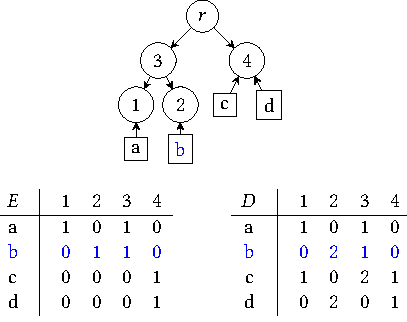
\includegraphics{figures/mutation_tree.pdf}

    \Description{A mutation tree with one root and four gene nodes, as well as four attached cells. Below, there are the corresponding true and noisy mutation matrices.}
    \caption{An example of a mutation tree, and related mutation matrices $E$ and $D$. The node $r$ represents the initial, unmutated state, the round nodes with numeric labels represent mutations of individual genes in the tree, and the square nodes with letter labels represent cells that are attached to the tree nodes. The true mutation matrix $E$ and the noisy mutation matrix $D$ have one row for each cell and one column for each gene. Exemplarily, the highlighted cell \textcolor{emph}{b} contains mutations in genes 2 and 3 (second row of $E$), but during readout, the information on gene 2 was lost (entry 2 in second row of $D$).}
    \label{fig:mutation_tree}
\end{figure}

%Even with this refined goal, there are still many possible versions of $E$. In order to restrict the possible true mutation matrices even further, 
In order to define a search space for plausible mutation matrices, the so-called "infinite sites assumption" is made in SCITE. It assumes that every gene mutates exactly once in the history of the tumor and that the first cell with such a mutation passes it down to all of its descendants that are created via cell division. This assumption allows to model the mutation history as a tree. Every node represents a mutation state and is labeled with a gene. The root $r$ represents the initial, unmutated state of the genome and every child adds a mutation of its label gene to its parent's state. In other words, a gene $g$ is mutated in the state of a node $v$ iff there is a node $w$ on the path from $r$ to $v$ with the label $g$. 
%Lastly, we attach our cells to nodes in the tree, which means that we assume the mutation state of the attachment node for this cell. 
During the cell-extraction process, samples from any node in the mutation tree can be encountered, which is modeled by attaching cells to tree nodes.
%The tree and the cell attachments together describe a candidate for $E$ which can be evaluated with the likelihood function. 
%Since we want to maximize the likelihood function, we always pick the most likely attachment node for every cell. 
Fig.~\ref{fig:mutation_tree} gives an example how of a mutation tree with respective $E$ and $D$ may look like. During the sequencing stage, errors are introduced from $E$ to $D$, and during the reconstruction phase, we look for an $E$ that has the highest likelihood w.r.t. to $D$ and at the same time can be modeled with a mutation history that forms a tree.
While $E$ is only completely defined by the combination of mutation tree and cell attachment, \ac{SCITE} actually explores the candidate space for mutation trees and calculates the likelihood of each tree by identifying the most likely attachment for each cell in each evaluation step.

\subsection{Search Procedure}

%\ac{SCITE}, as stated earlier, is a \ac{MCMC} algorithm:
The search procedure to explore candidate mutation trees is a \acf{MCMC}.
It starts with a randomly generated tree and iteratively applies random modifications to it. If the resulting tree, together with the most likely attachments, is more likely to be correct than the previous tree, it is accepted as the new solution. If the new tree is less likely to be correct, a random threshold between 0 and 1 is drawn. If the ratio of the proposed likelihood to the current likelihood is lower than this threshold, the modification is rejected. This kernel loop of modifying the tree, computing its likelihood, and deciding on the new solution is then repeated multiple times and also restarted with new trees. For statistical details on the convergence of this search procedure, we refer to \citeauthor{tree2016} \cite{tree2016}. %\todo{is this interesting at this point?} Note that in their implementation, the moves are performed via pointer operations on a tree data structure, which is then transformed into a so-called ancestor matrix in every step to calculate the likelihood.

%With every step, the current tree converges to the most likely solution. For the statistical details, see \citeauthor{tree2016} \cite{tree2016}.
